\documentclass[letterpaper, 10 pt, conference]{ieeeconf}  % Comment this line out
                                                          % if you need a4paper
%\documentclass[a4paper, 10pt, conference]{ieeeconf}      % Use this line for a4
                                                          % paper

\IEEEoverridecommandlockouts                              % This command is only
                                                          % needed if you want to
                                                          % use the \thanks command
\overrideIEEEmargins
% See the \addtolength command later in the file to balance the column lengths
% on the last page of the document

\usepackage[utf8]{inputenc}
\usepackage[T1]{fontenc}
\usepackage{graphicx}
\usepackage{float}
\usepackage{xcolor}
\usepackage{booktabs}
\usepackage{pgfgantt}
\usepackage{xcolor}
\usepackage[utf8]{inputenc}

\definecolor{barblue}{RGB}{153,204,254}
\definecolor{groupblue}{RGB}{51,102,254}
\definecolor{linkred}{RGB}{165,0,33} 
\usepackage{hyperref}
\hypersetup{
    colorlinks=true,
    linkcolor=blue,
    filecolor=magenta,      
    urlcolor=blue,
}
\overrideIEEEmargins

\title{Smart Sprinkler System with Real Time Feedback}
\author{Patrick Armstrong, Ryan Williamson, Caleb Edwards\\
    \textit{Dept. of Electrical and Computer Engineering, University of Utah}
}

\date{February 2020}

\begin{document}

\maketitle

\begin{abstract}
Watering a lawn is a common activity for every house owner. Deciding how long and at what time someone should water their lawn can vary depending on where a lawn is located and what kind of weather is in that location. This project is intended to solve the problem of time and length for watering a lawn through automated systems. By using using sensor arrays and remotely accessible sprinkler controller this project will automatically suggest when and for how long a lawn should be watered. A user will have full control via an online user-interface on whether to accept the suggestions by the system or to completely ignore them. This proposal outlines the the design and implementation of a Smart Sprinkler system with real-time feedback.

% OLD ABSTRACT
%Smart sprinkler irrigation control designed with Python and I2C using Raspberry Pi's, sensors, relay board, ESP32 micro-controller and a mobile/desktop interface that allows a user to schedule watering with real time feedback from moisture, weather and infrared sensors. Minimizing excess water usage with automated adjustments to reschedule watering zones based on real-time data.

\end{abstract}

\section{Introduction}
Watering and taking care of a lawn has been a task that has been around for many years. This seems like a project that should be well implemented and have many solutions. There should be a lot of competition in this field with how many people are using sprinkler controllers to water their yards. As of now, a person with a sprinkler controller has to go to their sprinkler box in their garage and manually enter times and duration for each zone in their yard. Not many people are sure how long or what time of day they should even water their yard. It is almost an educated guess for most people with controllers. Based off of these times and duration settings that are manually entered, the old controller will turn on and water that zone for the specified duration. We would like to make the controller smarter.

This project will be a smart sprinkler controller based off of different weather sensors placed throughout a user's yard. There are multiple zones controlled by one valve box and each valve box is controlled by the sprinkler controller. A zone is a subsystem in a sprinkler system that is controlled from a valve box, and there can be many valve boxes depending on the size of the yard and system. The goal of this project is to provide real time feedback to the user to make informed decisions on when and for how long to water each zone. Our main objective coming into this project was to create something that was feasible and stayed within budget for regular users of sprinkler systems.

Our system will be based on recommendations sent to the user through an user interface. There will be sensors that collect data throughout the day and get stored in our controller. The controller will have a time series database that records all these values. Based on these results, a predictive algorithm that we will create will send a recommendation to the UI stating a duration and time that the user should water that zone. The user will then be able to accept these recommendations, stick with the default settings, or enter some manual settings based on their preference. 

The controller will collect data from a hub station that will represent a weather station, as well as all the other systems in each zone. This will allow the user to also have that extra functionality on their system, viewed through the UI. The weather station could have sensors that relate to temperature, humidity, wind speed, etc. So if a user would like to base their input to the controller based on these results, they can do so. Each zone of the sprinkler system will have different sensors, including a moisture sensor placed in the dirt of that zone. The data fed to the controller from these results are how the recommendations are determined for unique times of each zone. The block diagram of how data will be transferred can be seen in Fig. 2.

\section{Background}
This project will be based off of a lot of open source material that are already available on the web \cite{SIP}. This project will have a UI that allows any user who has access to view data collected, and make decisions off of that. The difference between this project and other open source projects is that our system is based on recommendations. Based on the data that the system collects, a recommendation will be sent to the UI. The user will then have the option to change settings in the controller based on these recommendations, or leave them as they were. This project is about leaving control to the user. This system will not take over and do everything for the user, unless it is specified that the user wants that. A user could have a setting that says "Accept all recommendations", which would have the controller do everything for the user, but the user still has all the control in choosing that option. 

This project is running with a Raspberry Pi as the main controller, which is similar to many other examples \cite{SIP}. These computers have a lot of processing power, as well as memory that is located in SD cards placed externally on the board. This is what allows for adding a database and UI deployment in this project. The Raspberry Pi 3+ has four USB ports and an HDMI port. This allows us to flash Linux OS onto the Pi and then we can add the rest of the features from there, including the database, UI, etc. 

%%% Patrick add time series db here *****************************************************

\begin{figure}[H]
    \centering
    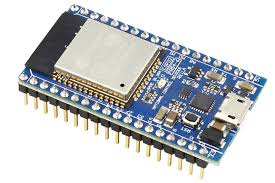
\includegraphics[scale=.5]{ESP32.jpg}
    \caption{ESP32 with Bluetooth and Wifi capabilities.}
    \label{fig:my_label}
\end{figure}

Many of these systems like the option to add sensors to help deliver accurate information on whether the lawn should be watered \cite{OpenSprinkler}. This project will have multiple sensors attached to an ESP32. This chip allows for wireless communication and can be programmed with MicroPython or Arduino. This is why it is used in many wireless communication projects \cite{OpenSprinkler}. These chips have an I2C bus for the sensors, and then can send that data over a wireless communication. This can be done with Wifi or Bluetooth, and a visual of the chip is found in Fig. 1. This chip provides a 240 MHz clock with around 512 MB of RAM \cite{Micropython}. This chip could offload some of the processing requirements of the Raspberry Pi onto itself if the situation required. That is what makes these chips so desirable. 

\begin{figure*}
	\centering
	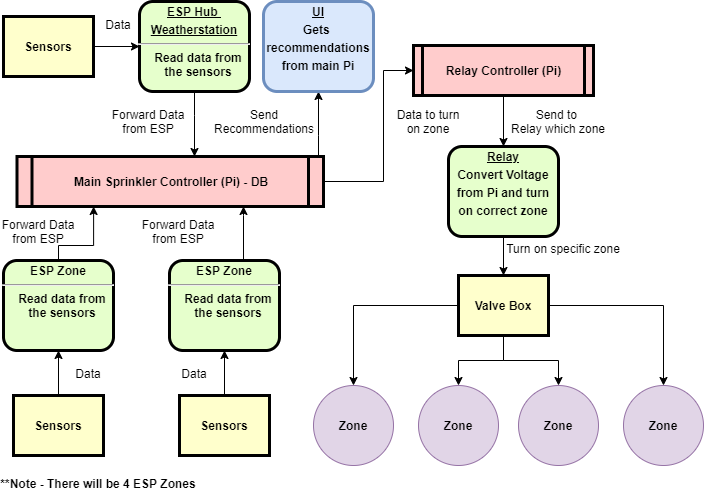
\includegraphics[width=\textwidth]{Diagram.png}
	\caption{Block Diagram of Sprinkler Controller}
	\label{label1}
\end{figure*}


\section{Project Tasks and Integration}
There will be many different tasks involved in the creation of a smart sprinkler system. Below we will specify the different tasks needed for this project, including their difficulty and how we will be testing of each of them.

\subsection{Sensor Arrays}
Sensors were selected based on two criteria: I2C protocol and cost. Providing relevant metrics such as light, temperature, soil ph, soil moisture and composition of the soil. Our product doesn't require a large area of precision, therefore one to two sensors per zone will suffice for accurate readings. Sensor data collection will be toggled by our micro controller (ESP32); whenever a measurement is needed. Storing up to five of the most previous read values for each individual sensor. We can reduce the power consumption of sensors by gathering data in timed intervals.

\subsection{Communication Between ESP and Sensors}
For this task, we will have the ESP32 that needs to read data given by a set of sensors. The ESP chip has an I2C bus for communication. Due to this aspect, we will only have sensors with I2C buses as well. The ESP will be running Micropython, and have an associated .py script that will read the I2C bus. This is described in \cite{LowCostBLE}. The data that the ESP now has stored will be sent to our main controller, which will be described in the next subsection.

Communication testing with sensors and the ESP will happen with testing one sensor at a time. Each sensor will be tested one at a time using the I2C bus, and validated that data can be read in different environments. This will be done to make sure that different data can be read in different scenarios, and that the sensor can be used in the final version of the project. Once this is completed, and all sensors have been validated, integration of the sensors can take place. This means that we will have multiple sensors sending data over the I2C bus to the ESP. We will start with two slaves to one master, and increase the slaves as we have more success. As soon as all sensors are added over I2C, this part of testing is done. 

\subsection{Communication Between ESP and Raspberry PI}
Once the ESP has the data from the sensors, the data needs to be transferred to the Pi for processing. This will be done with BLE communication. This part of the project will require a lot more effort and research as wireless communication is no easy task. Bluetooth is a big protocol and will be risky in trying to implement in our project. A tutorial that we will base this can be found in \cite{micropy}. If this does not work as planned, we will move to Wifi. We can accomplish this by following Wifi protocol, and examples found in \cite{rasServer}. Our last resort, if no wireless communication is possible, would be to transfer data over USB. This is the most simple, and the Pi has four USB ports for the four ESP's that we would be using.

Testing for communication between the Pi and the ESP will be opposite from what was stated in section 2. We will start with USB testing, and move on from there. As soon as the data is transferred from USB to USB, wireless testing will commence. BLE testing will happen first. This will be done by following the tutorial in \cite{micropy} as well as any other sites that might be found later on in development. If the BLE ends up not working by the October deadline, Wifi testing will begin. This will be done by following the tutorial in \cite{rasServer} as well as any other sources found in development. If all wireless testing fails, we will move back to USB connections and use that as our communication between ESP and Pi. 

\subsection{User Interface}
Since, sprinkler systems are a universal tool we decided to use a free open source Sprinkler/Irrigation control software called SIP (Sustainable Irrigation Platform) \cite{SIP}. The core software is written in python and runs under linux and implements an intuitive user interface (UI) in javascript on mobile/desktop. 

\begin{figure}[H]
    \centering
    \includegraphics[scale=.32]{RaspberryPIB.jpg}
    \caption{Raspberry Pi 3 Model B+}
    \label{fig:my_label}
\end{figure}

Most importantly SIP was developed and tested on raspberry pi models B,A and Zero. Reducing the risk and time investment of creating a UI for our product. It also provides a very large community of guides and resources for creating an irrigation control system interface with relay boards using raspberry pi's. We will use the interface to display data, provide improvements and give user control over zones and scheduling. We chose to do this, because we wanted to move away from the traditional control box. Creating a user-friendly interface for scheduling watering zones and providing feedback to maximize water usage.

The user interface shouldn't require much testing because it is an open source project that has been tested over a long period of time. We will have to adjust the interface to meet our requirements such as adding three new tabs for displaying the sensor data we collect. The interface will be very useful for testing and displaying data from our sensors and scheduling protocols. SIP provides a tutorial for connecting SainSmarts relay board which is capable of controlling other AC or DC devices such as sprinkler valves. The majority of interface testing will be done through the use of the application and fine tuning bugs/changes.



\subsection{Database and Data Storage}
Our projects open source sprinkler/irrigation control software, SIP \cite{SIP},has the capabilities of performing http get/post requests to manipulate or control SIP. The logging in feature that's included with SIP is disabled by default, in order to prevent the uncontrolled accumulation of log data. The raspberry pi controlling the SIP will utilize its memory on board for one user. By default, only 100 records will be recorded at a time. Upon the maximum number of records being reached, new records will be added to the top of the list and the oldest record will be deleted from the bottom. Archiving the records can be done through the log page which contains a link for a user to download the log data as a spread sheet friendly, comma separated values, (csv) text file to another device such as a laptop. Allowing us to keep permanent archived sprinkler data in manageable chunk sizes.
A separate database will be created using MySQL and python as needed. Containing any excess data the initial controllers memory was unable to hold.


\subsection{Predictive Algorithm}
There needs to be an algorithm that determines what happens with the data that is stored on the Pi. This could be done with a certain percentage given to each sensor that is read from each of the zones. Based on these percentages, an algorithm could determine a watering time for that zone, as well as a proposed watering time. These calculations are determined based on the sensors being a temperature, moisture, and other sensors listed on the bill of materials. Depending on how much data the user has, a machine learning model could be used for this project as well. This would be dependent on if the Pi had enough processing power to run machine learning algorithms, and contain a model. The model could be trained with previous summer's data, and then be used to determine predictions for the user. If time, data, and memory permits, a model will be trained based on the data and implemented to take future data and predict recommendations for the user. 

This portion of testing will be mostly trial and error. Based on the data, and how much we have of it, will determine what the algorithm produces. This algorithm will also be based off of past research \cite{SmartSprinkler}. There is really no wrong to the algorithm, as it is based on the data that has been collected in a certain area. For example, the moisture sensor will most likely have the highest percentage to determine output. Depending on how much moisture is in the soil, will determine that percentage of time that the specific zone needs watering. The watering time might be determined from real-time data, while the time of day of watering might be determined from historical data as well as real-time data. 

\subsection{Relay to Turn on Zones}
The relay board plugin from SIP \cite{SIP} allows a user to use one or more relay boards to control sprinkler valves; up to 12 stations. A variety of relay boards can be driven by a Raspberry Pi to turn sprinkler valves on. They are commonly available with 1, 2, 4, 8 and 16 channels. As for our relay board, we chose to use SainSmart's \cite{relayBoard} 4-channel 5v relay board (link for part in table 1). This board is active low, meaning a relay is switched on when the Raspberry Pi output changes from 3.3 Volts to 0 Volts.

The average valve in a sprinkler system requires a 24VAC signal to open, however a Raspberry Pi only outputs signals at a maximum of 5VDC. To convert the 5VDC that the Pi can output to 24VAC you must use a relay board to change the signal. Once the signal can be converted and the Pi can open and close valves freely, a script can be created on the Pi to send signals to each relay to close and open on command. The relay board plugin from SIP \cite{SIP} allows a user to use one or more relay boards to control sprinkler valves; up to 12 stations. A variety of relay boards can be driven by a Raspberry Pi to turn sprinkler valves on. They are commonly available with 1, 2, 4, 8 and 16 channels. As for our relay board, we chose to use SainSmart's \cite{relayBoard} 4-channel 5v relay board (link for part in table 1). 'This board is active low, meaning a relay is switched on when the Raspberry Pi output changes from 3.3 Volts to 0 Volts.'

To test the Pi and the relay together we will first use a simple python script to activate a I/O pin on the Pi to activate the relay to see if the valve opens and closes. Once it has been confirmed that a single signal works we will expand the amount of connections and expand the python script to receive input on when to shut and close the valves.


\subsection{Integration}
Once we have data from the sensors being read by the ESP, and valid communication from the Pi and the ESP; we will be able to integrate these tasks into data being read from the ESP and transferred to the Pi. This will then allow for testing on the predictive algorithm. Once we have data onto the Pi, we can test the algorithm to see if we have results that make sense from the data that we are actually reading. 

\section{Risk Assessment}
\subsection{Sensor Arrays}
Med Risk: We will be testing and collecting data for temperature, infrared and moisture sensors over the summer. Once we finalize our choice on sensors, we will build a sensor array for collecting and processing the signals. Ideally, all our sensors will operate on I2C and we should be able to efficiently grab data. Our real risk, lays in how effective and accurate our sensors produce data.

\subsection{Communication Between ESP and Sensors}
High Risk : The risk for this task is high because there can be multiple sensors trying to communicate with one ESP microcontroller. To mitigate this risk, one sensor will be added at a time. This will allow for steady progress when trying to add sensors as we move through the project and get to our final destination. Sensors that communicate with I2C will be sought after, since this is what ESP uses. This will lower the risk as we will not have to use different protocols with different sensors.

\subsection{Communication Between ESP and Raspberry PI}
High Risk : The risk for communication between the ESP and sensors is high. This is high due to the choice of using wireless communication. This will be done either with BLE or Wifi. To lessen the risk of this task, wired communication over I2C will be used. This will create a more stable and reliable communication that we are already used to. 

\subsection{User Interface}
Med/Low Risk: The interface is based upon an open source irrigation control system that is being actively updated and used. This interface however doesn't support our sensors and I will have to add it to the interface, thus the only true area of risk for this is whether or not we can add new sensor information.

\subsection{Database and Data Storage}
Med/Low Risk: Will use a raspberry pi with MySQL and python to create and manage our database. This will be used to hold user data from sensors.However, MySQL and python are very simplistic to work with and shouldn't give any troubles.

\subsection{Predictive Algorithm}
Low Risk: The algorithm is low risk due to the fact that if we cannot find verified or supported information on the data that we receive, then we can create our own custom algorithm. The algorithm will work no matter what, but it might not be as efficient as we would want it to be. This is what makes it low risk. The algorithm will work, but efficiency could be limited.

\subsection{Relay to Turn on Zones}
Low/Med Risk: We are using a Raspberry Pi 8-Relay Card add-on which is supported with our open source interface and has low risk given its universal usage and correlation with the Raspberry PI Model 3 A+.

\section{Communication Plan and Schedule}
Our group communication plan consists of two different platforms. We will use Discord for real time, fast communication. We will use Github for the management of all tasks and document storage. 

Discord will be for all of our immediate communication. If we have a time pressing question that needs to be discussed, Discord allows real time communication. Discord also allows file sharing if the team needs to view something in that exact moment \cite{discord}.

Github will allow us to all have access to our repository, as well as view the project plan and tasks associated with this repo. The project portion of Github allows you to use a Kanban style management for the agile project management. This process will allow us to view the progress of each other to see if we are falling behind in different areas. This will allow us to manage our time and help others with certain tasks if we realize we are falling behind \cite{github}. 

During the semester we plan on meeting at least once a week to discuss how things are progressing. If one member is having trouble with a task, this time can be used to meet in person to resolve the problem. The time at which we meet each week will be flexible based on everyone's schedules the upcoming semester.

\subsection{Spring}
\begin{itemize}
    \item Finish initial design/research. - Team
    \item Finish and submit project proposal. - Team
    \item Start interface development. - Ryan
\end{itemize}

\subsection{Summer}
\begin{itemize}
    \item Connect sensors to Pi for testing - Team
    \item Collect data using chosen sensors - Team
    \item ESP testing - Caleb
\end{itemize}

\subsection{August}
\begin{itemize}
    \item Interface finished and testing - Ryan
    \item Get relay working with Pi to activate valves - Patrick
    \item Create algorithms per sensor - Team
\end{itemize}

\subsection{September}
\begin{itemize}
    \item Finalize sensors to use - Team
    \item Finalize Database layout - Team
    \item Build sensor arrays - Ryan and Patrick
    \item Integrate all parts with wired communications - Team
    \item Start developing wireless communication - Caleb
\end{itemize}

\subsection{October}
\begin{itemize}
    \item Combine algorithms together - Team
    \item Build sprinkler demo - Team
    \item Want wireless to be finished - Caleb
\end{itemize}

\subsection{November}
\begin{itemize}
    \item Wireless fully integrated - Caleb
    \item Demo tested - Team
    \item Touch-up/bug testing - Team
    \item Finish Documentation - Team
\end{itemize}

\subsection{December}
\begin{itemize}
    \item Present Project - Team
\end{itemize}



\section{Parts and Vendor List}
\subsection{Sensors}
\begin{itemize}
  \item BME280/680 (Temp/Humidity/Pressure)
  \item DHT22 (Temp/Humidity)
  \item BH1750 (Light)
\end{itemize}

\subsection{Communications/Compute/Electronic Boards}
\begin{itemize}
  \item 1-2x Raspberry Pi 3 B+
  \item 1x Raspberry Pi Zero W
  \item 4-5x ESP32
  \item Channel Relay Board
\end{itemize}

\subsection{Sprinkler Equipment}
\begin{itemize}
  \item 4x Sprinkler Valves
\end{itemize}

Links are provided for each vendor for quick access to purchase parts and provide more information. See table 1 below for links to each parts page.
\begin{table}[hbt!]
\resizebox{0.45\textwidth}{!}{%
    \begin{tabular}{}
        \begin{tabular}{|c|c|c|}
        \hline
        Vendor 1 & Vendor 2 & Item \\
        \hline
        \hline
        \href{https://www.amazon.com/Adafruit-BME280-Temperature-Humidity-Pressure/dp/B013W1AJUY}{Adafruit(280)}& \href{https://www.adafruit.com/product/3660}{Adafruit(680)} & BME280/680 \\
        \hline
         \href{https://www.adafruit.com/product/385}{Adafruit} &\href{https://www.adafruit.com/product/381}{Adafruit(DS18B20)} & DHT22 \\
        \hline
        \href{https://www.dfrobot.com/product-531.html}{DFRobot} & \href{https://www.amazon.com/RobotDyn-Photosensitive-digital-Raspberry-projects/dp/B073RBS2N5}{RobotDyn} & BH1750 \\
        \hline
      \href{https://www.raspberrypi.org/products/raspberry-pi-3-model-b-plus/}{Raspberry Pi} & \href{https://www.adafruit.com/product/3055#technical-details}{Adafruit} & Raspberry Pi 3 B+ \\
        \hline
        \href{https://www.raspberrypi.org/products/raspberry-pi-zero/}{Raspberry Pi} &\href{https://www.sparkfun.com/products/14277}{Sparkfun} & Raspberry Pi Zero W \\
        \hline
        \href{https://www.amazon.com/HiLetgo-ESP-WROOM-32-Development-Microcontroller-Integrated/dp/B0718T232Z}{HiLetgo} & & ESP32 \\
        \hline
        \href{https://www.sainsmart.com/products/4-channel-5v-relay-module}{Sain Smart} & \href{https://wiki.52pi.com/index.php/DockerPi_4_Channel_Relay_SKU:_EP-0099}{52Pi} & Relay Board \\
        \hline
       \href{https://www.whiteboxes.ch/shop/i2c-soil-moisture-sensor/}{WhiteBoxLabs} & \href{https://www.adafruit.com/product/381}{Adafruit} & I2C Soil Sensor \\
        \hline
        \end{tabular}
   \end{tabular}%
   }
   \caption{"List of Vendors and Items with links"}
\end{table}

Many of the secondary vendors for the parts are links provided for other options besides those listed above in the bill of materials.
\section{Conclusion}
The spring and summer milestones can be completed independently of each other, with no integration at that time. When the fall months arrive, integration testing starts having to take place and dependencies occur. For the month of August, we will need data to determine the algorithm. By September, the database and algorithm should be completed. This will allow the Pi to access the database and compute the algorithm. The UI will also need to be completed by September so the recommendations can be sent to the user. By October, we will need the relay to work, the communication between sensors and ESP, and the USB communication between Pi and ESP to all be ready to go. These will have to be integrated to start with a completed UI and database to see if the project can fully come together. The relay will have to work so the recommendations that the user selects can be implemented and shown from the relay. At this point the rest of the project will have to come together for final testing. 

The main high risks that come from this project come from the communication end. The communication from the Pi to the ESP is high risk while it is wireless. This risk turns medium when one node can communicate with the Pi. After this, it will be trying to make all nodes communicate clearly with the Pi. This risk becomes low, after individual testing is completed. The risk won't be as high when having to integrate. Or if this fails, the risk is low if we have to use USB connections. The communication between the ESP and the sensors is the next risk that needs to be evaluated. This risk will turn low when all sensors have been decided and tested together with an ESP. The risk will be lowered to medium when each sensor has been tested and verified individually. 

There are many people with brown, dead yards. There grass does not get enough water, or they over water their yards. Sprinklers get left on and a lot of water is wasted. This project fixes those problems. This will automate and predict the best time of day to water your yard, as well as determine and predict the length of time your yard should be watered. It will display to the UI the recommendations that have been determined and let the user decide on if these recommendations seem valid. This system provides help to the users, without taking the control away from the user. 


\bibliographystyle{IEEEtran}
\bibliography{bibliography}

%\begin{thebibliography}{99}
%\bibitem{c1} https://discordapp.com/
%\bibitem{c2} https://github.com/
%\bibitem{c3} https://dan-in-ca.github.io/SIP/
%\end{thebibliography}

\end{document}
